\section{Continuous Training and Serving} \label{continuous-training-serving}
\todo[inline]{text not polished, but structure is complete}
\todo[inline]{add algorithm for continuous training}
In this section, we describe our continuous deployment approach.
We describe optimization technique for training the model and how we utilize it to work in hybrid environment.
We also provide detailed description of how we implement each of the proposed optimizations (proactive training and statistics collections).

\subsection{Stochastic Gradient Descent} \label{sgd}
\textit{Stochastic Gradient Descent (SGD) } is a optimization strategy used by many machine learning algorithms for training a model.
SGD is an iterative optimization algorithm where in each iteration a sample of the data is used to make updates to the model.
It works well in presence of large datasets \cite{bottou2010large}, as it does not require scanning the entire data in every iterations.
SGD is has been used in many machine learning algorithms and tasks.
SGD is used in different classification \cite{zhang2004solving} tasks to build logistic regression models for Ads click rate prediction \cite{macmahan2013}.
It is in clustering \cite{bottou1995convergence} to build k-means clustering models.
It is used in matrix factorization \cite{funk2006netflix} to build recommender systems  \cite{koren2009matrix}. .
And it is used in neural networks \cite{dean2012large} for training the networks on large datasets.
Some recent examples of SGD in neural networks are Google deepmind that managed to train a NN that defeat humans in the game of Go  \cite{silver2016mastering} and mastering Atari games \cite{mnih2013playing} .

In our example application, a logistic regression model is trained using the SGD optimization method \cite{macmahan2013}.
In logistic regression, the goal is to find the vector ($w$ that maximizes the conditional likelihood of labels ($y$) based on the given data ($x$) in the training dataset,

$w^* = \argmin_w ln[\prod_{i=1}^{N} P(y^i | x^i, w)]$

To use SGD to find the optimal $w$, we start from an initial random weights and in each step make small updates based on the gradient of the loss function. 

${w}^{t+1} = {w}^t + \eta \sum_{i \in S} x^i [y^i - \hat{P}(Y^i = 1 | x^i w)]$

where $\eta$ is the learning rate parameter and $S$ is the random sample in the current iteration.
The algorithm continues until convergence (weight vector does not changes).

\textbf{Learning Rate. }
A very important parameter of stochastic gradient descent is the learning rate adaptation technique. 
Learning rate controls the degree to which in each iteration SGD the weights are updated.
Momentum \cite{qian1999momentum}, Adam \cite{kingma2014adam}, RMSPROP \cite{tieleman2012lecture}, and AdaDelta \cite{zeiler2012adaptive} are the most effective learning rate tuning methods for stochastic gradient descent. 
Moreover, some of the methods perform per coordinate modification. 
This is important because not all the parameters of the model contribute the same way and some changes more rapidly based on the training data.

\textbf{Sample Size}
Another parameter of stochastic gradient descent is the sample size.

\textbf{Distributed SGD. }
To efficiently train machine learning models on large datasets, scalable techniques have to be employed.
SGD inherently works well with large amounts of data because it does not need to scan every data point during every iteration.
However, for very large datasets, SGD has to perform many iterations in order to converge.
To decrease the running time, large datasets can be distributed among multiple nodes, where each node will compute the gradients on a subset of the data in parallel.
One drawback of this approach is that a synchronization step is required before applying the updates to the model, which slows down the optimization process.
To alleviate this, several asynchronous SGD methods are proposed \cite{recht2011hogwild, dean2012large}. 
Experiments show that in certain cases asynchronous SGD performs well and the final quality of the model is comparable with the synchronous approach.

\subsection{Proactive Training}
We use the iterative nature of SGD in the design of continuous deployment process.
Iterations of SGD are independent.
We use this to schedule iterations and execute them while the prediction requests are being answered.
However, the two parameters of SGD (learning rate and sample size) play an important role.
They have to be tuned to increase the efficiency of the training.
In our experiment we show that which learning rate adaptation technique works the best.
The existing learning rate adaptation techniques either study the effect in a batch environment or in streaming environment.
However, in our deployment system the pipelines are trained both in batch and real-time therefore the effect of the learning rates should be studied in the hybrid environment.
Some the methods also adapt to the batch sizes and control the step size accordingly.
We have to pay attention to the step size as updating the model parameter by a large amount while doing real-time streaming may lower the accuracy of the predictions.
We also perform different sampling methods (random and weighted).
In our experiment we show that what are the most useful sampling technique.
The size of the sample also plays an important role the quality and total overhead on the system.
We study the effect of sampling rate on both of these metrics in the evaluation as well.
To increase the efficiency of the system a scheduler component is designed that is tasked with scheduling new iterations of SGD.
The new iterations are scheduled based on the rate of the incoming data.


\subsection{Statistics Collection}
To increase the efficiency of offline training we collect statistics while the system is running.
Whenever new training data arrives at the system they will pass through a component that will scan the incoming data and update the incoming statistics.
Statistics required can be defined by the pipeline.
In chapter \ref{sec:system-architecutre} we describe how the system exposes an API that allows both proactive training and statistics collection.
These statistics can then be used for training the pipeline.
The statistics basically come free since the data has to be scanned for training anyway.
The statistics can also be exported for use outside of the system.
There are cases that changes have to be made to the existing pipeline or new components should be added.
In these cases the pipeline is manually retrained.
Statistics related to the dataset collected while the system was running can be used to speed up the offline training of the pipeline.

\subsection{Improved Example Application}
\todo[inline]{without statistics collection unit, prediction is affected because new categorical examples may appear that are disregarded}
\todo[inline]{add statistic collection unit}
Figure \ref{fig:improved-example} shows how our deployment approach improves the example application described in section \ref{introduction}.
After the training of the initial model \textcircled{A}, it is deployed in the deployment environment \textcircled{B}.
Prediction requests are send by the user to the deployment environment \textcircled{1} where based on the current model for each ad a score is predicted\textcircled{2}.
Based on the score a few ads are shown to the user \textcircled{3}.
Depending whether or not the user clicks on them, feedback are send back to the deployment system \textcircled{4}.
Similar to current approaches the data is stored in the click log database.
However, contrary to existing methods, the data is routed to the deployment system immediately.
The data is first used to update the statistics for the pipeline.
After which the data is appended with a sample of the data stored in the click log.
Based on this new dataset an iteration of SGD is performed which updates the logistic regression model on the spot.
The updates are available immediately and as a result any new prediction requests that arrive at the system will predicted by a more up-to-date model.

\begin{figure}[t]
\centering
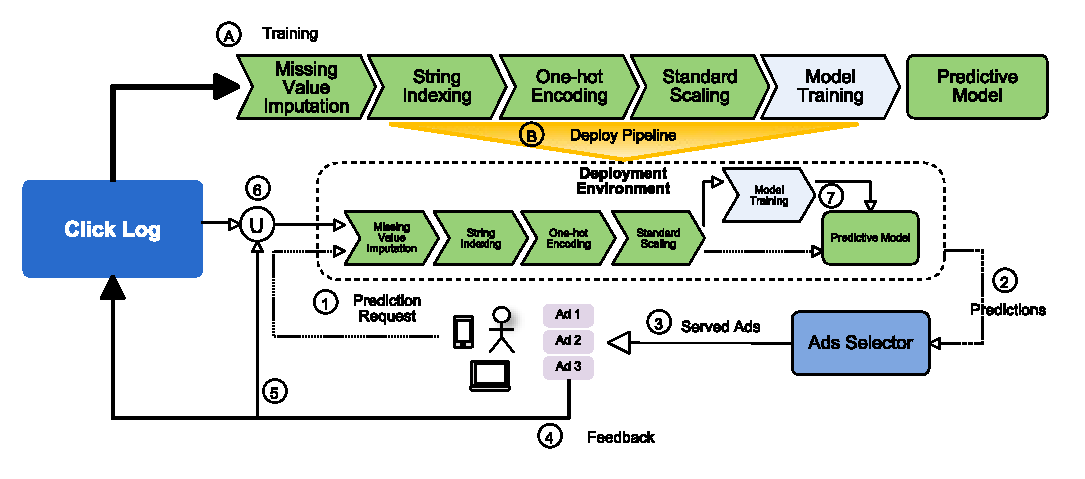
\includegraphics[width=\columnwidth]{../images/improved-example.pdf}
\caption{Ads Serving Continuous Training}
\label{fig:improved-example}
\end{figure}

